\chapter{Функции обработчика прерывания от системного таймера}
Обработчик прерываний от системного таймера имеет наивысший приоритет. 
Никакая другая работа в системе не может выполняться во время обработчика прерывания от системного таймера. 
Обработчик прерывания от системного таймера должен завершаться как можно быстрее, чтобы не
влиять на отзывчивость системы (отзывчивость показывает, насколько быстро система отвечает на запросы пользователей).

Основные определения: 

\textbf{Тик} - период времени между двумя последующими прерываниями таймера.

\textbf{Основной тик} - период времени равный N тикам таймера (число N зависит от конкретного варианта системы).

\textbf{Квант времени (quantum, time slice)} — временной интервал, в течение которого процесс может использовать процессор до вытеснения другим
процессом.

\section{UNIX}
\subsection*{По тику}
\begin{itemize}
	\item инкремент счетчика тиков аппаратного таймера;
	\item инкремент часов и других таймеров системы;
	\item инкремент счетчика использование процессора текущим процессом (то есть инкремент поля p\_cpu структуры proc до максимального
	значения – 127);
	\item декремент кванта текущего потока;
	\item декремент счетчика времени до отправления на выполнение отложенных вызовов, 
	при достижении счетчиком нуля происходит выставление флага для обработчика отложенного вызова
\end{itemize}

\subsection*{По главному тику}
\begin{itemize}
	\item пробуждает в нужные моменты системные процессы, такие как swapper и pagedaemon. (”пробуждает” тут понимается так: регистрация отложенного вызова процедуры wakeup, которая перемещает дескрипторы процессов из списка ”спящие” в очередь ”готовых к выполнению”);
	\item инициирование отложенного действия по выполнению функций, относящихся к работе планировщика, путём посылки сигнала {\ttfamily SIGCONT}, обработчик которого изменяет состояние процесса со {\ttfamily Sleep} на {\ttfamily Running};
	\item декрементирует счетчик времени, которое осталось до отправления одного из следующих сигналов:
	\begin{enumerate}
		\item SIGPROF – сигнал, посылаемый процессу по истечении времени заданного в таймере профилирования;
		\item SIGALRM – сигнал, посылаемый процессу по истечении времени, предварительно заданного функцией alarm().
		\item SIGVTALRM – сигнал, посылаемый процессу по истечении времени, заданного в “виртуальном” таймере;
	\end{enumerate}
\end{itemize}

\subsection*{По кванту}
\begin{itemize}
	\item посылает текущему процессу сигнал SIGXCPU, если он превысил
	выделенную для него квоту использования процессора. По получению
	сигнала обработчик сигнала прерывает выполнение процесса.
\end{itemize}


\section*{Windows}
\subsection*{По тику}
\begin{itemize}
	\item инкремент счетчика системного времени;
	\item декремент счетчиков времени отложенных задач;
	\item декремент кванта текущего потока на величину, равную количеству тактов процессора, произошедших за тик;
	\item если активен механизм профилирования ядра, то инициализация отложенного вызова обработчика ловушки профилирования ядра с помощью постановки объекта в очередь DPC (обработчик ловушки профилирования регистрирует адрес команды, выполнявшейся на момент прерывания);
\end{itemize}

\subsection*{По главному тику}
\begin{itemize}
	\item Освобождение объекта «событие», которое ожидает диспетчер настройки баланса. (Диспетчер настройки баланса по событию от таймера сканирует очередь готовых процессов и повышает приоритет процессов, которые находились в состоянии ожидания дольше 4 секунд.)
\end{itemize}

\subsection*{По кванту}
\begin{itemize}
	\item Инициация диспетчеризации потоков (добавление соответствующего
	объекта в очередь DPC ( Deferred procedure call — отложенный вызов
	процедуры));
\end{itemize}


\chapter*{Пересчет динамических приоритетов}
В ОС семейства UNIX и в ОС семейства Windows могут динамически пересчитываться приоритеты только
пользовательских процессов.

\section*{UNIX}
Планирование процессов в UNIX основано на приоритете процесса. 
Планировщик всегда выбирает процесс с наивысшим приоритетом. 
Приоритеты процессоров изменяются с течением времени (динамически) системой в зависимости от использования вычислительных ресурсов, времени ожидания запуска и текущего состояния процесса. 
Если процесс готов к запуску и имеет наивысший приоритет, планировщик приостановит выполнение текущего процесса (с более низким приоритетом), даже если тот не «выработал» свой временной квант.

Традиционное ядро UNIX является строго невытесняющим, однако в современных системах UNIX ядро является вытесняющим – то есть процесс в режиме ядра может быть вытеснет более приоритетным процессом в режиме ядра.
Ядро сделано вытесняющим для того, чтобы система могла обслуживать процессы реального времени, например работу с видео и аудио.

Очередь процессов, готовых к выполнению, формируется согласно приоритетам и принципу вытесняющего циклического планирования, то есть
сначала выполняются процессы с большим приоритетом, а процессы с одинаковым приоритетом выполняются в течении кванта времени друг за другом циклически. 
В случае, если процесс с более высоким приоритетом поступает в очередь процессов, готовых к выполнению, планировщик вытесняет текущий процесс и предоставляет ресурс более приоритетному процессу.

Приоритет процесса задается любым целым числом, которое лежит в
диапазоне от 0 до 127 (чем меньше число, тем выше приоритет):
\begin{itemize}
	\item 0 - 49 – зарезервированы для ядра (приоритеты ядра фиксированы);
	\item 50 - 127 – прикладные (приоритеты прикладных задач могут изменяться во времени);
\end{itemize}

Изменение приоритета прикладных задач зависит от следующих факторов:
\begin{itemize}
	\item \textbf{фактор ”любезности” (nice)} -- это целое число в диапазоне от 0 до 39 со значением 20 по умолчанию. 
	Увеличение значения приводит к уменьшению приоритета. 
	Пользователи могут повлиять на приоритет процесса при помощи изменения значений этого фактора, но
	только суперпользователь может увеличить приоритет процесса. 
	Фоновые процессы автоматически имеют более высокие значения этого фактора.
	\item степень загруженности процессора в момент последнего обслуживания им процесса.
\end{itemize}

Структура proc содержит следующие поля, которые относятся к приоритетам:

\begin{itemize}
	\item \textbf{p\_pri} -- текущий приоритет планирования;
	\item \textbf{p\_usrpri} -- приоритет режима задачи;
	\item \textbf{p\_cpu} -- результат последнего измерения использования процессора;
	\item \textbf{p\_nice} -- фактор ’любезности’, который устанавливается пользователем
\end{itemize}

\textbf{p\_pri} используется планировщиком для принятия решения о том, какой процесс отправить на выполнение.

\textbf{p\_pri} и \textbf{p\_usrpri} равны, когда процесс находится в режиме задачи.
Значение \textbf{p\_pri} может быть изменено (повышено) планировщиком для того, чтобы выполнить процесс в режиме ядра. 
В таком случае \textbf{p\_usrpri} будет использоваться для хранения приоритета, который будет назначен
процессу при возврате в режим задачи.

\textbf{p\_cpu} инициализируется нулем при создании процесса (и на каждом тике обработчик таймера увеличивает это поле текущего процесса на 1, до
максимального значения равного 127).
Ядро системы связывает приоритет сна с событием или ожидаемым ресурсом, из-за которого процесс может блокироваться (приоритет сна определяется для ярда, поэтому лежит в диапазоне 0 - 49). 
Когда процесс ”просыпается”, ядро устанавливает в поле \textbf{p\_pri} приоритет сна – значение приоритета из диапазона системных приоритетов, зависящее от события или ресурса по которому произошла блокировка.

В таблице 1.1 приведены приоритеты сна в ОС 4.3 BSD.

\begin{table}[h]
	\caption{Системные приоритеты сна в ОС 4.3 BSD}
	\begin{center}
		\begin{tabular}{| c | c | c |} 
			\hline
			\textbf{Приоритет} & \textbf{Значение} & \textbf{Описание}\\
			\hline
			PSWP & 0 & {Свопинг} \\
			\hline
			{PSWP + 1} & 1 & {Страничный демон}\\
			\hline
			{PSWP + 1/2/4} & 1/2/4 & {Другие действия по обработке памяти} \\
			\hline
			{PINOD} & 10 & {Ожидание освобождения inode}\\
			\hline
			{PRIBIO} & 20 & {Ожидание дискового ввода-вывода}\\
			\hline
			{PRIBIO + 1} & 21 & {Ожидание освобождения буфера}\\
			\hline
			{PZERO} & 25 & {Базовый приоритет}\\
			\hline
			{TTIPRI} & 28 & {Ожидание ввода с терминала}\\
			\hline
			{TTOPRI} & 29 & {Ожидание вывода с терминала}\\
			\hline
			{PWAIT} & 30 & {Ожидание завершения процесса потомка} \\
			\hline
			{PLOCK} & 35 & {Консультативное ожидание блок. ресурса}\\
			\hline
			{PSLEP} & 40 & {Ожидание сигнала}\\
			\hline
		\end{tabular}
	\end{center}
\end{table}

Также на рисунке 1 приведена таблица системных приоритетов сна из книги ”Операционная система UNIX” Андрея Робачевского.
\FloatBarrier
\begin{figure}[h]
	\begin{center}
		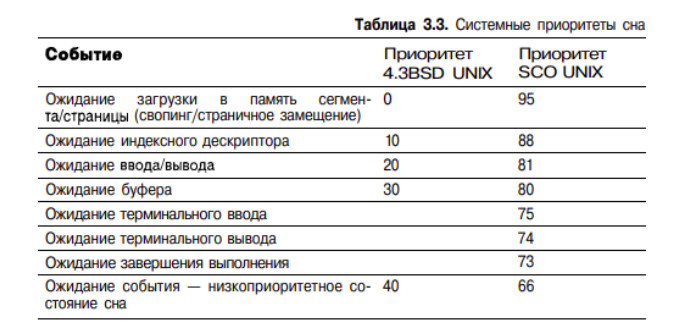
\includegraphics[]{inc/rob.png}
	\end{center}
	\caption{Системные приоритеты сна}
\end{figure}
\FloatBarrier

Каждую секунду ядро системы инициализирует отложенный вызов процедуры schedcpu(), которая уменьшает значение p\_pri каждого процесса исходя из фактора ”полураспада”. Расчёт производится по формуле 2.1:
\begin{equation}
 {decay} = \frac{2 * {load\_average}}{2 * load\_average + 1}
\end{equation}

где load\_average - это среднее количество процессов, находящихся в состоянии готовности к выполнению, за последнюю секунду.

Также процедура schedcpu() пересчитывает приоритеты для режима задачи всех процессов по формуле 2.2:
\begin{equation}
{decay} = {PUSER} + \frac{{p\_cpu}}{2} + 2 * {p\_nice}
\end{equation}

где PUSER - базовый приоритет в режиме задачи, равный 50.

Таким образом, если процесс в последний раз использовал большое количество процессорного времени, то его р\_срu будет увеличен. 
Это приведет к росту значения p\_usrpri, то есть к понижению приоритета. 
Чем дольше процесс простаивает в очереди на выполнение, тем больше фактор полураспада уменьшает его р\_срu, что приводит к повышению его приоритета. 
Такая схема предотвращает бесконечное откладывание низкоприоритетных процессов. 
Применение данной схемы предпочтительно процессам, осуществляющим много операций ввода-вывода, в противоположность процессам, производящим много вычислений.

То есть, если процесс большинство времени выполнения тратит на ожидание ввода-вывода, то он остается с высоким приоритетом и, таким образом, быстрее получает процессор при необходимости.
В тоже время вычислительные приложения обычно обладают более высокими значениями р\_срu и работают на значительно более низких приоритетах.

\textbf{Динамический пересчет приоритетов процессов в режиме задачи позволяет избежать бесконечного откладывания.}

Таким образом, приоритет процесса в режиме задачи может быть динамически пересчитан по следующим причинам:
\begin{itemize}
	\item Вследствие изменения фактора любезности процесса системным вызовом nice;
	\item В зависимости от степени загруженности процессора процессом p\_cpu;
	\item Вследствие ожидания процесса в очереди готовых к выполнению процессов;
	\item Приоритет может быть повышен до соответствующего приоритета сна вследствие ожидания ресурса или события.
\end{itemize}

\section*{Windows}
В Windows реализуется приоритетная, вытесняющая система планирования, при которой всегда выполняется хотя бы один работоспособный (готовый) поток с самым высоким приоритетом, с той оговоркой, что конкретные, имеющие высокий приоритет и готовые к запуску потоки могут быть
ограничены процессами, на которых им разрешено или предпочтительнее всего работать.
В Windows планировка потоков осуществляется на основании приоритетов готовых к выполнению потоков. 
Поток с более низким приоритетом вытесняется планировщиком, когда поток с более высоким приоритетом становится готовым к выполнению.

Код Windows, отвечающий за планирование, реализован в ядре. Нет единого модуля или процедуры с названием ”планировщик”, так как этот
код рассредоточен по ядру. 
Совокупность процедур, выполняющих эти обязанности, называется диспетчером ядра. 
Диспетчеризация потоков может быть вызвана в случаях:
\begin{itemize}
	\item поток готов к выполнению (только что создан или вышел из состояния ”ожидания”);
	\item поток выходит из состояния ”выполняется”, т.к. его квант истек, либо поток завершается, либо переходит в состояние ”ожидание”;
	\item поменялся приоритет потока;
	\item изменилась привязка к процессорам, следовательно, поток больше не может работать на процессоре, на котором он выполнялся.
\end{itemize}

Windows использует 32 уровня приоритета:
\begin{itemize}
	\item от 0 до 15 – 16 изменяющихся уровней (из которых уровень 0 – зарезервирован для потока обнуления страниц);
	\item от 16 до 31 – 16 уровней реального времени;
\end{itemize}
Уровни приоритета потоков назначаются исходя из двух разных позиций: одной от Windows API и другой от ядра Windows.
Сначала Windows API систематизирует процессы по классу приоритета, который им присваивается при создании:

\begin{itemize}
	\item Реального времени — Real-time (4);
	\item Высокий — High (3);
	\item Выше обычного — Above Normal (7);
	\item Обычный — Normal (2);
	\item Ниже обычного — Below Normal (5);
	\item Простоя — Idle (1)
\end{itemize}

После назначается относительный приоритет отдельных потоков внутри этих процессов:

\begin{itemize}
	\item Критичный по времени — Time-critical (15);
	\item Наивысший — Highest (2);
	\item Выше обычного — Above-normal (1);
	\item Обычный — Normal (0);
	\item Ниже обычного — Below-normal (–1);
	\item Самый низший — Lowest (–2);
	\item Простоя — Idle (–15).
\end{itemize}
Исходный базовый приоритет потока наследуется от базового приоритета процесса. 
Процесс по умолчанию наследует свой базовый приоритет у того процесса, который его создал. 
Соответствие между приоритетами Windows API и ядра системы приведено в таблице 1.2.


\begin{table}[h]
	\caption{Системные приоритеты сна в ОС 4.3 BSD}
	\begin{center}
		\begin{tabular}{| c | c | c | p{45pt} | c | p{45pt} | c |} 
			\hline
			& \textbf{real-time} & \textbf{high} & \textbf{above normal} & \textbf{normal} & \textbf{below normal} & \textbf{idle} \\
			\hline
			\textbf{time critical} & 31 & 15 & 15 & 15 & 15 & 15 \\
			\hline
			\textbf{highest} & 26 & 15 & 12 & 10 & 8 & 6 \\
			\hline
			\textbf{above normal} & 25 & 14 & 11 & 9 & 7 & 5 \\
			\hline
			\textbf{normal} & 24 & 13 & 10 & 8 & 6 & 4 \\
			\hline
			\textbf{below normal} & 23 & 12 & 9 & 7 & 5 & 3 \\
			\hline
			\textbf{lowest} & 22 & 11 & 8 & 6 & 4 & 2 \\
			\hline
			\textbf{idle} & 16 & 1 & 1 & 1 & 1 & 1 \\
			\hline
		\end{tabular}
	\end{center}
\end{table}

Текущий приоритет потока в динамическом диапазоне – от 1 до 15 – может быть повышен планировщиком вследствие следующих причин:
\begin{itemize}
	\item \textbf{Повышение вследствие событий планировщика или диспетчера (сокращение задержек)}
	
	При наступлении события диспетчера вызываются процедуры с целью проверить не должны ли на локальном процессоре быть намечены какие-либо потоки, которые не должны быть спланированы. 
	При каждом наступлении такого события вызывающий код может также указать, какого типа повышение должно быть применено к потоку,
	а также с каким приращением приоритета должно быть связано это повышение.
	
	\item \textbf{Повышения приоритета, связанные с завершением ожидания}
	
	В общем случае поток, пробуждающийся из состояния ожидания, должен иметь возможность приступить к выполнению как можно скорее.
	\item \textbf{Повышение приоритета владельца блокировки}
	
	Так как блокировки ресурсов исполняющей системой и блокировки критических разделов используют основные объекты диспетчеризации, 
	то в результате освобождения эих блокировок осуществляются повышения приоритетв, связанные с завершением ожидания. 
	Но с другой строны, так как высокоуровневые реализации этих объектов отслеживают владельца блокировки, то ядро может принять решение
	о том, какого вида повышение должно быть применено с помощью AdjustBoost.
	
	\item \textbf{Повышение вследствие завершения ввода-вывода}
	
	Windows дает временное повышение приоритета при завершении определенных операций ввода/вывода, при этом потоки, которые ожидали ввода/вывода имеют больше шансов сразу же запуститься. Подходящее значение для увеличения зависит от драйвера устройств (представлены в таблице 1. 3).
	\FloatBarrier
	\begin{table}[h]
		\caption{Рекомендуемые значения повышения приоритета}
		\begin{center}
			\begin{tabular}{| p{245pt} | p{100pt} |}
				\hline
				\textbf{Устройство} & \textbf{Приращение} \\
				\hline
				Диск, CD-ROM, параллельный порт, видео & 1 \\
				\hline
				Сеть, почтовый ящик, именованный канал,
				последовательный порт & 2 \\
				\hline
				Клавиатура, мышь & 6 \\
				\hline
				Звуковая плата & 8 \\
				\hline
			\end{tabular}
		\end{center}
	\end{table}
	\FloatBarrier
	\item \textbf{Повышение при ожидании ресурсов исполняющей системы}
	
	Если поток пытается получить ресурс исполняющей системы, который уже находится в исключительном владении другого потока, то
	он должен войти в состояние ожидания до тех пор, пока другой поток не освободит ресурс. 
	Для ограничения риска взаимных исключений исполняющая система выполняет это ожидание, не входя в бесконечное ожидание ресурса, а интервалами по 500 мс.
	Если по окончании этих 500 мс ресурс все также находится во владении, то исполняющая система пытается предотвратить зависание
	центрального процессора путем получения блокировки диспетчера, повышения приоритета потока (потоков), владеющих ресурсом до 15
	(в случае если исходный приоритет владельца был меньше, чем у ожидающего, и не был равен 15), перезапуска их квантов и выполнения еще одного ожидания.
	
	\item \textbf{Повышение приоритета потоков первого плана после ожидания}
	
	Смысл такого повышения заключается в улучшении скорости отклика интерактивных приложений, то есть если дать приложениям первого плана небольшое повышение приоритета при завершении ожидания, то у них повышаются шансы сразу же приступить к работе,
	особенно когда другие процессы с таким же базовым приоритетом могут быть запущены в фоновом режиме.
	
	\item \textbf{Повышение приоритета после пробуждения GUI-потока}
	
	Потоки — владельцы окон получают при пробуждении дополнительное повышение приоритета на 2 из-за активности при работе с окнами, например, при поступлении сообщений от окна. Система работы с окнами ( Win32k.sys ) применяет это повышение приоритета, когда
	вызывает функцию KeSetEvent для установки события, используемого для пробуждения GUI-потока. 
	Смысл такого повышения схож со смыслом предыдущего повышения — содействие интерактивным приложениям.
	
	\item \textbf{Повышения приоритета, связанные с перезагруженностью центрального процессора}
	
	Диспетчер настройки баланса (механизм ослабления загруженности центрального процессора) сканирует очередь готовых потоков раз в
	секунду и, если обнаружены потоки, ожидающие выполнения более 4 секунд, то диспетчер настройки баланса повышает их приоритет
	до 15. Как только квант истекает, приоритет потока снижается до базового приоритета. 
	Если поток не был завершен за квант времени или был вытеснен потоком с более высоким приоритетом, то после
	снижения приоритета поток возвращается в очередь готовых потоков.
	Диспетчер настройки баланса сканирует лишь 16 готовых потоков и повышает приоритет не более чем у 10 потоков (если найдет) за один проход. 
	При следующем проходе сканирование возобновляется с того места, где оно было прервано в прошлый раз.
	
	\item \textbf{Повышение приоритетов для мультимедийных приложений и игр}
	
	Потоки, на которых выполняются различные мультимедийные приложения, должны выполняться с минимальными задержками. 
	В Windows такая задача решается с помощью повышения приоритетов таких потоков драйвером MMCSS (MultiMedia Class Scheduler Service).
	MMCSS работает с различными определенным задачи, например:
	\begin{itemize}
		\item аудио;
		\item игры;
		\item захват;
		\item воспроизведение;
		\item задачи администратора многооконного режима;
		\item распределение.
	\end{itemize}
\end{itemize}

Важное свойство для планирования потоков – категория планирования
– это первичный фактор, который определяет приоритет потоков, зарегистрированных с MMCSS (категории планирования указаны в таблице 2.4).
Функции MMCSS временно повышают приоритет потоков, зарегистрированных с MMCSS до уровня, который соответствует категории планирования. 
Потом их приоритет снижается до уровня, соответствующего категории планирования Exhausted, для того, чтобы другие потоки тоже могли получить ресурс.

\begin{table}[h]
	\caption{Системные приоритеты сна в ОС 4.3 BSD}
	\begin{center}
		\begin{tabular}{| p{90pt} | c | p{245pt} |} 
			\hline
			\textbf{Категория} & \textbf{Приоритет} & \textbf{Описание}\\
			\hline
			{High (Высокая) } & 23-26  & {Потоки профессионального аудио
				(Pro Audio), запущенные с приоритетом выше, чем у других потоков
				на системе, за исключением критических системных потоков} \\
			\hline
			{Medium (Средняя)} & 16-22  & {Потоки, являющиеся частью приложений первого плана, например
				Windows Media Player}\\
			\hline
			{Low (Низкая)} & 8-15 & {Все остальные потоки, не являющиеся частью предыдущих категорий} \\
			\hline
			{Exhausted (Исчерпавших потоков)} & 1-7 & {Потоки, исчерпавшие свою долю
				времени центрального процессора,
				выполнение которых продолжиться,
				только если не будут готовы к выполнению другие потоки с более высоким уровнем приоритета}\\
			\hline
		\end{tabular}
	\end{center}
\end{table}


\chapter*{Вывод}
Функции обработчика прерывания от системного таймера в защищенном режиме для ОС семейства UNIX и для OC семейства Windows схожи. 

Общие основные функции:
\begin{itemize}
	\item декремент кванта текущего процесса в UNIX и декремент текущего потока в Windows.
	\item инициализация отложенных действий, которые относятся к работе планировщика (например пересчет приоритетов).
	\item декремент счетчиков времени (таймеров, часов, счетчиков времени отложенных действий, будильников реального времени).
\end{itemize}

Обе системы являются системами разделения времени с динамическими приоритетами и вытеснением.